%%%%%%%%%%%%%%%%%%%%%%%%%%%%%%%%%%%%%%%%%%%%%%%%%%%%%%%%%%%
% EPFL report package, main thesis file
% Goal: provide formatting for theses and project reports
% Author: Mathias Payer <mathias.payer@epfl.ch>
%
% To avoid any implication, this template is released into the
% public domain / CC0, whatever is most convenient for the author
% using this template.
%
%%%%%%%%%%%%%%%%%%%%%%%%%%%%%%%%%%%%%%%%%%%%%%%%%%%%%%%%%%%
\documentclass[a4paper,11pt,oneside]{report}
% Options: MScThesis, BScThesis, MScProject, BScProject
\usepackage[MScThesis,lablogo]{EPFLreport}
\usepackage{xspace}

\title{Framework for Evaluating Synthetic Drivers for Library Fuzzing}
\author{Zurab Tsinadze}
\supervisor{Dr. sc. Flavio Toffalini}
\adviser{Prof. Dr. sc. ETH Mathias Payer}
%\coadviser{Second Adviser}
% \expert{The External Reviewer}

\newcommand{\sysname}{FooSystem\xspace}



\usepackage{listings}
\usepackage{color}
\usepackage{xcolor}

\definecolor{dkgreen}{rgb}{0,0.6,0}
\definecolor{gray}{rgb}{0.5,0.5,0.5}
\definecolor{mauve}{rgb}{0.58,0,0.82}

\lstdefinestyle{DOS}
{
    backgroundcolor=\color{black},
    basicstyle=\scriptsize\color{white}\ttfamily,
}


\lstset{frame=tb,
  language=c++,
  aboveskip=3mm,
  belowskip=3mm,
  showstringspaces=false,
  columns=flexible,
  basicstyle={\small\ttfamily},
  numbers=none,
  numberstyle=\tiny\color{gray},
  keywordstyle=\color{blue},
  commentstyle=\color{dkgreen},
  stringstyle=\color{mauve},
  breaklines=true,
  breakatwhitespace=true,
  tabsize=3
}
\lstset{escapeinside={<@}{@>}}



\begin{document}
\maketitle
% \makededication
% \makeacks

% The abstract serves as an executive summary of your project.
% Your abstract should cover at least the following topics, 1-2 sentences for
% each: what area you are in, the problem you focus on, why existing work is
% insufficient, what the high-level intuition of your work is, maybe a neat
% design or implementation decision, and key results of your evaluation.
\begin{abstract}

The software contains bugs or defects that can potentially allow unauthorized
access to our data or enable attackers to escalate their privileges, such as
by installing malware. Various testing strategies exist to help developers
identify these bugs before they can cause any harm. One effective strategy is
fuzzing, which involves executing a program in a controlled test environment
with random inputs to detect crashes.

While fuzzing binaries, such as CLI programs, can be easily done with a
single click using out-of-the-box solutions, library fuzzing requires testers
to tackle an additional level of complexity: it is essential to have drivers
that make use of the APIs exposed by the library. However, developing drivers
that are semantically correct and have high coverage is a time-consuming and
a technically challenging task that typically requires a deep understanding 
of the library.

Several research efforts have focused on automating driver generation. The 
objective of this project is to investigate the current state of the art in
this field, and create methodology and tooling for evaluating automatically
generated drivers.

\end{abstract}

% \begin{frenchabstract}
% For a doctoral thesis, you have to provide a French translation of the
% English abstract. For other projects this is optional.
% \end{frenchabstract}

\maketoc


%%%%%%%%%%%%%%%%%%%%%%
\chapter{Introduction}
%%%%%%%%%%%%%%%%%%%%%%
Complex software systems are susceptible to various types of input-based bugs.
Some of these bugs might be vulnerabilities that can be exploited by the 
adversary to gain unauthorized access, execute arbitrary code, or mount
a denial-of-service (DoS) attack. 

Fuzzing is a software testing technique that involves executing the 
program with random inputs to catch vulnerabilities and bugs. The idea behind
the technique is simple, it stresses the program with a large number of diverse
inputs. These inputs could be random (black box fuzzing) or could be generated 
by mutating previous "interesting" (according to some metric, such as code
coverage) inputs. Coverage-guided mutational fuzzing is considered to be
state-of-art.

Fuzzing has been on the rise in the last couple of years and is currently 
commonly used across the industry and many open-source projects, including libraries. 

Fuzzing binaries is considered much easier compared to libraries due to several factors.
When fuzzing binary, the tester focuses on the executable file itself, they can directly
target the file, which usually has a well-defined entry point, such as the main function, 
which is the ideal point to inject inputs for fuzzing. Binaries usually have a predictable
input format: often accept CLI arguments, files, network packets, or some other 
well-structured input. Moreover, binaries generally do not have state management complexity.

On the other hand, fuzzing libraries requires additional considerations. Libraries
are developed to be reusable, serving different purposes for different applications. 
Testers need to manually define and implement entry points, or so-called drivers.
The drivers act as the interface between the fuzzing engine and the library.
They need to be carefully designed, taking into account multiple different factors
that we will discuss in the next chapter.

While it may involve more effort and consideration compared to fuzzing binaries, 
thoroughly testing libraries is extremely important, since popular libraries 
are used across different software applications, making any vulnerability in them
highly impactful and widespread, giving attackers an opening to exploit all consumer
software (think of Log4j vulnerability \cite{log4j}). By fuzzing libraries, potential 
security risks can be identified and addressed early in the software 
development life-cycle, reducing the likelihood of vulnerabilities being exploited in production.

Google operates numerous online services and, just like the whole industry, 
heavily relies on various open-source software components. With the goal
of improving the overall security and stability of open-source projects,
they started the OSS-Fuzz project \cite{ossfuzz}. They provide automated fuzzing
infrastructure, tools, and even computational resources to allow "important" 
projects (open to interpretation, but as a rule-of-thumb, it needs to be critical
for the global IT world or have a large user base) to integrate fuzzing into their CI pipeline. 
As of June 2023, there are 1087 projects in OSS-Fuzz and the project has helped identify and 
fix over 8,900 vulnerabilities and 28,000 bugs \cite{ossfuzz-trophies}.

While OSS-Fuzz undoubtedly reduces the burden on library developers
by providing all the tooling, there is still room for improvement. An ideal
scenario would be to automate the process of writing drivers, reducing or 
even completely removing the effort required from developers.
Automating the driver generation has immense potential in enhancing the
efficiency of library fuzzing. By removing this step, developers can save
time and resources and instead focus on rolling-out new features or
analyzing and fixing bugs and vulnerabilities. 
An automated approach to driver generation would involve leveraging
program analysis techniques to analyze APIs and codebase in general. This analysis could identify 
key entry points, function signatures, input requirements, inter-dependencies of APIs,
and expected behaviors, allowing the automated tool to generate semantically correct 
and effective fuzzing drivers.
By automating the driver generation process, library developers could 
seamlessly integrate fuzzing into their development workflows, promoting 
continuous security testing and proactive vulnerability discovery. 
This automation would not only reduce the burden on library developers 
but also ensure a more systematic and comprehensive approach to 
library fuzzing, ultimately leading to improved software security and stability.

The topic of automating the generation of drivers for library fuzzing
has attracted attention in recent research works. Several papers have
been proposed with various techniques, such as program analysis,
analysis of how consumers use the libraries, and large language models.

The goal of this project is to create a framework and methodology for
evaluating the effectiveness of these tools and comparing them with drivers
manually written by developers of the libraries. This evaluation would 
allow us to understand the strengths and limitations of these tools. 
Furthermore, comparing automated and manual drivers shows their relative 
performance and effectiveness in terms of code coverage achieved, 
bug discovery rate, and time and effort required. 
It helps determine whether automated drivers can provide comparable 
results to their manual counterparts and identify areas for improvement 
or optimization, the insight that could be used while designing similar tools.





% Provide an overview of existing research and techniques in library fuzzing.
% Discuss different approaches to library fuzzing, such as manual driver creation and automatic driver generation.
% Highlight the advantages and disadvantages of each approach.
%%%%%%%%%%%%%%%%%%%%
\chapter{Background}
%%%%%%%%%%%%%%%%%%%%
This section aims to provide the necessary context and knowledge
of the technologies used in this project, discuss the challenges associated with 
library fuzzing, and present related work in synthetic driver generation.


\section{Fuzzing}
The intuition behind fuzzing lies in mutating or generating 
inputs that are then fed into the program being tested. 
By subjecting a program to a wide range of inputs, fuzzing helps 
identify and address potential security flaws, stability issues, and unexpected behavior.
Mutation-based fuzzing involves taking initial inputs (also known as corpus) 
and applying various modifications, such as bit flips, random insertions, deletions, or replacements, 
to create a mutant. By exploring the program's behavior with 
these inputs, fuzzing aims to trigger crashes. These crashes are saved for human analysis.
While "interesting" inputs are added to the corpus.

Due to its randomness, the core goal of the fuzzing is to execute 
the program with different inputs as many times as possible considering 
a limited amount of resources, both time and CPU. However, there is always 
a trade-off between the speed and efficiency of fuzzing. 
Black box fuzzers treat the program as a black box, apply random mutations to the inputs, 
and collect as many crashes as possible. Coverage-guided grey box 
fuzzing, on the other hand, uses feedback obtained from code 
coverage analysis during the fuzzing process. This technique aims 
to guide the fuzzing process toward uncovering deeper program states. 
It instruments the program under test to collect coverage information 
during execution and uses this feedback to guide the generation of new inputs. 
By utilizing coverage information, coverage-guided grey box fuzzing tends 
to be more effective at finding complex vulnerabilities and exploring deeper
program states. Figures \ref{fig:blackbox_diag} and \ref{fig:coverage_guided_diag}
demonstrate the difference between the two techniques. 


\begin{figure}[ht]
	\centering
	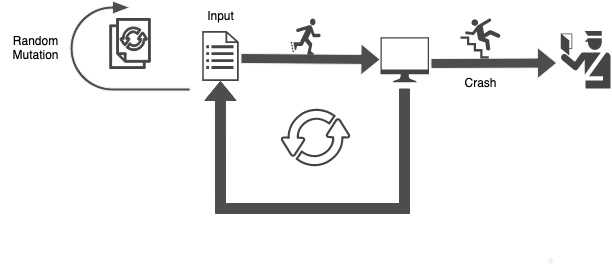
\includegraphics[width=12cm]{figures/black_box.png}
	\caption{Black Box fuzzing}
	\label{fig:blackbox_diag}
\end{figure}

\begin{figure}[ht]
	\centering
	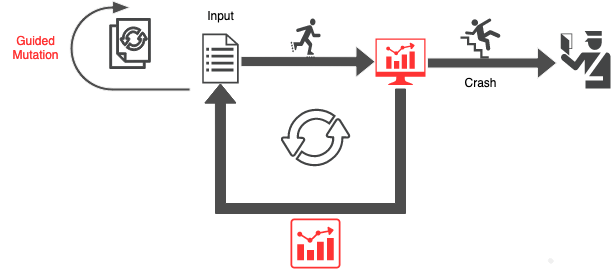
\includegraphics[width=12cm]{figures/coverge_guided_red.png}
	\caption{Coverage-guided Greybox fuzzing}
	\label{fig:coverage_guided_diag}
\end{figure}


Fuzzing engines focus on capturing inputs that cause program crashes, 
but they may miss inputs that trigger bugs but do not result in a crash. 
For instance, scenarios like out-of-bounds reads or writes may not 
cause a crash. This is where sanitizers play a crucial role.

\section{Sanitization TODO: might remove this section}

Sanitizers are oracles that mark a bug. They instrument programs compile-time
by adding different checks to enforce policies during run-time. 
Sanitization helps identify issues such as memory errors or leaks (ASan), uninitialized
memory reads (MSan), undefined behavior (UBSan), and data races (TSan)
that can be potential security vulnerabilities.
Violation of these policies results in a crash that will be saved by the fuzzing engine,
sanitizers make faults detectable. 
By integrating sanitizers into the fuzzing process, the fuzzer can detect 
and report errors more effectively. However, Careful consideration is 
required when selecting the appropriate sanitizer for fuzzing, 
as the core principle of fuzzing revolves around speed and efficiency. 
Sanitizers, while immensely valuable for detecting memory-related bugs, 
come with significant run-time costs, often resulting in performance 
slowdowns ranging from 2 to 10 times. Additionally, compatibility 
issues arise when multiple sanitizers are combined, leading to an 
exponential increase in slowdowns for each added sanitizer. 
Given these constraints, it becomes crucial to prioritize the selection 
of sanitizers that align with the specific goals of the fuzzing process. 
Since a substantial portion of bugs typically involve memory-related issues \cite{memorysafety2} \cite{memorysafety1}, 
it often makes sense to utilize AddressSanitizer (ASan) due to its effectiveness 
in detecting memory errors. To see ASan in action consider the following simple code snippet:

\lstset{caption={}, label=asan}
\begin{lstlisting}[language={c++}]
#include <iostream>

void parseInput(const char *input) {
  char buffer[10];
  strncpy(buffer, input, sizeof(buffer) - 1);
  buffer[sizeof(buffer) - 1] = '\0';
  std::cout << "Value at index 20: " << buffer[20] << std::endl;
}

int main() {
  const char *input = "This is long input string";
  parseInput(input);
  return 0;
}
\end{lstlisting}

If we compile this code with no sanitizer flags and run it, we would get 
an output that looks something like this: \lstinline{Value at index 20: ?}, where `'?'' is some
garbage value. However, compiling it with \lstinline{-fsanitize=address} flag will
result in a crash: TODO: where the fuck do these white lines come from

\lstset{caption={}, label=asan-crash}
\begin{lstlisting}[style=DOS]
=================================================================
<@\textcolor{red}{==38533==ERROR: AddressSanitizer: stack-buffer-overflow on address 0x00016d at pc 0x000102 bp 0x00016d}@>
READ of size 1 at 0x00016d69f154 thread T0
    #0 0x102761184 in parseInput(char const*)+0x1d4 (asan:arm64+0x100001184)
    #1 0x1027615a0 in main+0x28 (asan:arm64+0x1000015a0)
    #2 0x1ab44fe4c  (<unknown module>)
Address 0x00016d69f154 is located in stack of thread T0 at offset 52 in frame
    #0 0x102760fbc in parseInput(char const*)+0xc (asan:arm64+0x100000fbc)
  This frame has 1 object(s):
    [32, 42) 'buffer' <== Memory access at offset 52 overflows this variable
SUMMARY: AddressSanitizer: stack-buffer-overflow in parseInput(char const*)+0x1d4
...
==38533==ABORTING
\end{lstlisting}





\section{Library Testing}

\subsection{Challenges with the Library Fuzzing}

As previously mentioned, libraries are designed for the reusability 
across various applications and for serving different purposes. 
Unlike binaries, they do not have a well-defined entry point, 
posing a challenge for testers. To bridge the gap between the fuzzing 
engine and the library, testers must manually create drivers—code 
snippets that facilitate interaction with the library. These drivers 
serve as the interface through which the fuzzing engine interacts 
with the library's functionality. There are multiple challenges
associated with writing such drivers.

\begin{enumerate}
  \item Understanding of the library: Testers should have good knowledge of intended usage,
  APIs, and functionality. This is crucial for identifying key entry points and relevant
  target functions for fuzzing.
  \item Input Semantics: While the fuzzing engine will handle generating semi-random inputs,
  testers should split this data into different parts to fuzz different parameters. These
  chunks should adhere to API's expected formats. 
  \item Starting Seeds: Testers need to select initial inputs, known as seeds, to effectively
  jumpstart the fuzzing process. The quality and diversity of these seeds play a crucial
  role in the effectiveness of the fuzzing campaign. However, selecting seeds for libraries
  can be more challenging compared to binaries.
  \item Callback Handling: Libraries oftentimes have callbacks that require testers
  to implement appropriate handling in the drivers. 
  \item Error Handling: Drivers should have error handling mechanisms to gracefully 
  handle exceptions, crashes, or any other unexpected behavior during fuzzing. Drivers
  should not crash.
  \item State Management: Libraries have stateful behavior and testers need to manage
  internal state appropriately. This involves initializing the library, setting necessary
  configurations, and ensuring the state is reset on each fuzz input run. This is extremely 
  important for in-process fuzzing engines.
\end{enumerate}


For synthetic fuzz drivers to be considered on par with manually written ones,
they need to effectively address the majority of these challenges. 
To understand the complexity of this requirement, let us have a look at the following code:
\\
\\

\lstset{caption={Open tiff file, read metadata, read image data, close the file}, label=libtiff}
\begin{lstlisting}[language={c}]
#include <stdio.h>
#include <tiffio.h>

void errorHandlingCallback(const char* module, const char* format, va_list args) {
    vfprintf(stderr, format, args);
}

void processImageData(TIFF* tiff, uint32_t width, uint32_t height) {
    uint16_t bitsPerPixel, samplesPerPixel;
    TIFFGetField(tiff, TIFFTAG_BITSPERSAMPLE, &bitsPerPixel);
    TIFFGetField(tiff, TIFFTAG_SAMPLESPERPIXEL, &samplesPerPixel);
    uint32_t imageSize = width * height * (bitsPerPixel / 8) * samplesPerPixel;
    unsigned char* imageData = (unsigned char*)malloc(imageSize);
    if (imageData) {
        TIFFReadRGBAImage(tiff, width, height, (uint32_t*)imageData, 0);
        // Process the image data as needed
        free(imageData);
    }
}

void processTIFFFile(const char* filename) {
    TIFF* tiff = TIFFOpen(filename, "r");
    if (tiff) {
        uint32_t width, height;
        // Retrieve image dimensions
        if (TIFFGetField(tiff, TIFFTAG_IMAGEWIDTH, &width) &&
            TIFFGetField(tiff, TIFFTAG_IMAGELENGTH, &height)) {
            // Process the image data
            processImageData(tiff, width, height);
        } else {
            fprintf(stderr, "Failed to retrieve image dimensions\n");
        }
        TIFFClose(tiff);
    } else {
        fprintf(stderr, "Failed to open TIFF file: %s\n", filename);
    }
}

int main() {
    TIFFSetErrorHandler(errorHandlingCallback);
    const char* filename = "example.tif";
    processTIFFFile(filename);
    return 0;
}
\end{lstlisting}


Even for arguably simple usage of the libtiff library, the provided code 
snippet demonstrates the complexity of creating the driver. The process of reading 
TIFF image files requires careful consideration of various factors and 
dependencies within the library. The correct usage requires opening the TIFF 
file using the \lstinline{TIFFOpen()} function and subsequently retrieving image metadata
information with multiple \lstinline{TIFFGetField()} calls. The \lstinline{TIFFReadRGBAImage()} function, 
responsible for reading the image data, depends on the successful execution of both 
\lstinline{TIFFOpen()} and \lstinline{TIFFGetField()} calls. The code also has 
important error-handling measures, such as checking for file opening and 
memory deallocation to prevent leaks. Moreover, the \lstinline{TIFFSetErrorHandler()} 
function expects a callback as the argument. This example shows the importance of 
careful handling and adherence to library-specific requirements.


\subsection{LibFuzzer}

LibFuzzer \cite{libfuzzer} is an \textbf{in-process}, coverage-guided, 
evolutionary fuzzing engine developed by Google that specializes in
library testing. 


LibFuzzer is a coverage-guided evolutionary fuzzing engine 
designed for in-process fuzzing. It is integrated with the 
library being tested and operates by feeding fuzzed inputs 
through a specific fuzzing entry point, also known as the "target function." 
As the fuzzing process unfolds, LibFuzzer tracks the code 
coverage achieved by the inputs and generates mutations on 
the existing corpus to maximize the coverage. The code coverage 
information utilized by LibFuzzer is provided by LLVM's SanitizerCoverage instrumentation.

To use LibFuzzer on a library, the first step is to implement 
a fuzz target function (or as we called it before - the driver). 
This function receives an array of bytes as input and performs 
interesting operations on the data using the library's API. 
The fuzzing engine executes the fuzz target multiple times 
with different inputs within \textbf{the same process}. 
The fuzz target should be tolerant of various input types, 
including empty, large, or malformed inputs. It should not \lstinline{exit()} 
on any input and ideally joins all threads within the function. 
The fuzz target should also strive for speed, avoiding complex operations, 
excessive memory consumption, and global state modifications. 
Narrower targets are preferred, with each target focused on a specific aspect or format.

Coverage-guided fuzzing heavily relies on a corpus of sample inputs. 
This corpus should be initialized with a diverse collection 
of valid and invalid inputs relevant to the code under test. 
For instance, in the case of a graphics library, the initial 
corpus might contain a variety of small PNG or JPG files. 
LibFuzzer generates random mutations based on these sample 
inputs, exploring new code paths in the process. If a mutation triggers 
the execution of a previously uncovered path, it is saved to the 
corpus for further mutations and added to the queue. 
The corpus also serves as a sanity and regression check, 
ensuring that the fuzzing entry point remains functional 
and that the sample inputs successfully pass through the 
code under test without encountering issues.

As you see, LibFuzzer's requirements for its target function
largely reassembles the challenges that we defined in the previous 
subsection.

\lstset{caption={LibFuzzer fuzz target signature}, label=libfuzzer}
\begin{lstlisting}[language={c++}]
extern "C" int LLVMFuzzerTestOneInput(const uint8_t *Data, size_t Size) {
  DoSomethingWithData(Data, Size);
  return 0;
}
\end{lstlisting}


Custom mutators and dictionaries are important features 
supported by LibFuzzer, enhancing the efficiency of fuzzing.

Custom mutators allow testers to define their own mutation 
functions tailored to the specific characteristics of the 
target library or input format. This enables the generation 
of more targeted and meaningful mutations, increasing the 
likelihood of discovering vulnerabilities or triggering 
specific code paths. Custom mutators can be designed to 
manipulate specific data structures, and modify certain 
fields or properties. Custom mutators can significantly 
improve the quality of the generated test cases.

Dictionaries, on the other hand, serve as a valuable 
resource for guiding the fuzzing process toward relevant 
and interesting areas of the code. A dictionary is 
a list of input values or keywords that have significance 
within the library's API or expected input format. 
By providing a dictionary to LibFuzzer, testers can 
bias the generation of test cases towards these predefined values, 
increasing the chances of triggering specific functionalities or 
exercising critical code paths. Dictionaries can be especially useful 
in situations where certain inputs or parameter values are 
known to have a significant impact on the behavior of the library. 
By focusing the fuzzing efforts on these important values, 
testers can efficiently explore the space of inputs and 
increase the likelihood of finding vulnerabilities or uncovering unexpected behaviors.
For instance, if we are fuzzing library that handles PNG files, triggering
some parts of the codebase might depend on the input file having so-called critical chunks: \textbf{IHDR},
\textbf{PLTE}, \textbf{IDAT}, and \textbf{IEND}.
A dictionary with these keywords would give us massive speedup as random 
bitflips will take a long time to produce them.


%%%%%%%%%%%%%%%%
\section{Related Works}
%%%%%%%%%%%%%%%%




The field of automatic driver generation for library fuzzing 
has seen significant advancements in recent years. Several 
notable works have emerged in top-tier conferences, including FuzzGen \cite{fuzzgen}, 
UTopia \cite{utopia}, FUDGE \cite{fudge}, and RUBICK \cite{rubick}.
These tools aim to automate the process of generating drivers 
that interact with libraries, enabling effective fuzzing campaigns. 
In order to evaluate the effectiveness of these automatic approaches, 
it is essential to compare them with manually written drivers,
which have traditionally been used for library fuzzing. 
For this purpose, we consider manually written drivers from the OSS-Fuzz project. 
By examining the strengths and weaknesses of both automatic 
and manual driver generation techniques, we can gain valuable 
insights into the advancements made in automatic driver generation.
This chapter presents the core ideas of related works.


\subsection{FUDGE}
FUDGE is a system designed to speed up the creation of 
fuzz drivers. While the drivers it generates still require 
some input and fixes from the tester, the tool's main concept 
is that it can automatically synthesize fuzz drivers that are 
semantically correct by analyzing how the target library is 
used in the existing codebase. FUDGE processes the entire 
Google codebase, including third-party libraries, 
searching for instances where the target library is 
utilized, extracting relevant information, and using 
it to create drivers. These generated fuzzers are then 
executed using LibFuzzer, and FUDGE filters out
uninteresting drivers based on their runtime behavior. 
The tool presents various metrics to the developer, 
such as code coverage, size of the generated driver, 
and observed crashes, through a UI. 
Developers can then adapt and modify the fuzz 
targets based on this feedback.

\begin{figure}[ht]
	\centering
	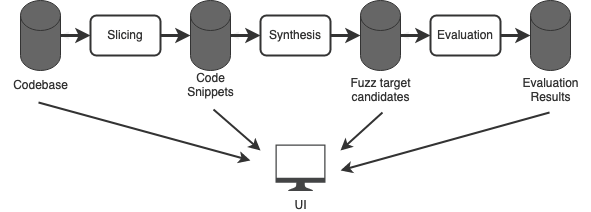
\includegraphics[width=12cm]{figures/fudge.png}
	\caption{High-level overview of the FUDGE.}
	\label{fig:fudge}
\end{figure}


\subsection{FuzzGen}
FuzzGen analyzes unit tests inside library and library consumers, 
i.e., programs or other libraries on a system (Android, Debian, etc.) 
that use the target library. The tool consists of three parts: an 
API inference, an \emph{Abstract API Dependence Graph} ($A^{2}DG$)
construction mechanism, and a driver generator that uses $A^{2}DG$. 

For the API inference, FuzzGen discovers all declared functions
in the library and all functions used in the system. The intersection
of these two sets gives us which functions of the library
are actually being used, everything else can be ignored.
The $A^{2}DG$ is a graph that records all API interactions, 
including parameter value range and possible interactions. 
Next, generic $A^{2}DG$ is constructed by merging different consumers.
The driver generator component leverages this $A^{2}DG$ 
to automatically synthesize fuzzers capable of building complex states.
FuzzGen then uses LibFuzzer to fuzz individual API components.

FuzzGen was developed concurrently and independently from FUDGE. 
While the core ideas behind these two projects might be similar, 
there are a few differences. Firstly, FUDGE extracts code snippets 
from a single consumer, and created drivers are then
tested dynamically. In contrast, FuzzGen iterates CFG, i.e., minimizing 
consumers. Secondly, FUDGE creates multiple small fuzz drivers from snippets,
while FuzzGen merges multiple consumers into single
$A^{2}DG$ allowing the synthesis of arbitrary length drivers 
(any random walk through this graph is a possible driver). 
FuzzGen drivers are larger and more generic, allowing 
to create complex API sequences.

\subsection{UTopia}
UTopia claims that both FuzzGen and FUDGE have fundamental 
limitation in their approach by relying on consumer code and instead
proposes to infer API dependencies by utilizing unit tests. 

The high-level idea of UTopia is to take the unit test, which has an API
calls with parameters in it, and convert it to fuzz driver by injecting 
fuzz inputs into some of the API parameters. UTopia runs a 
so-called root definition analysis to identify where it can 
inject inputs without affecting valid API usage semantics.

This approach has several advantages. 
\begin{enumerate}
  \item Large number of popular projects already have 
  well-written unit tests.
  \item Unit tests are written by library developers, 
  people who have knowledge of intended usage.
  \item Testers may use constant values as API parameters 
  inside unit tests. These values are extracted by UTopia
  and form an initial corpus.
  \item Usually unit tests have the so-called tearDown function
  that is run after each execution of the test. This function may 
  be used to ensure that the state, or at least part of it, is reset
  before each fuzz run.
\end{enumerate}

However, the majority of UTopia crashes are still spurious. Unit test
code is used for testing, developers do not intend to use it for 
executing it multiple times in-process. They will hard code non-
essential parameters and neglect error handling since the code is not
intended for production. 


\subsection{RUBICK}


To solve the challenges faced by previous related works, RUBICK
introduces an automata-guided control-flow-sensitive approach for
fuzz driver generation. It represents API usage as deterministic 
finite automata and utilizes an active automata learning algorithm 
to distill the API usage patterns. This information is then 
used to synthesize a single automata-guided fuzz driver, 
which provides a scheduling interface for the fuzzer. 
The fuzzer can use this interface to test independent 
sets of API usage during the fuzzing process. While the 
abstract of the paper suggests a promising idea and 
presents short evaluation results, it's important to note 
that the paper is currently under embargo until the 
32nd USENIX Security Symposium, and further details and 
findings are not yet publicly available.





% Explain the methodology you followed to conduct fuzzing campaigns.
% Describe the setup and configuration of your fuzzing environment.
% What tools were used for clustering, triaging, coverage
%%%%%%%%%%%%%%%%%%%%%%%%
\chapter{Methodology}
%%%%%%%%%%%%%%%%%%%%%%%%

In this chapter, we will introduce a semi-automatic framework and best 
practices for evaluating the quality of automatically generated drivers. 
The objective of this chapter is to provide a comprehensive overview of
the framework, highlighting key components. By employing our framework,
researchers can gain valuable insights into the performance, effectiveness, 
and potential limitations of the automatically generated drivers. 


\section{High Level description}
Our analysis has two parts: library analysis, which focuses on static information
obtained from the target library source code, and driver analysis, which involves
dynamic metrics gathered during the execution of the generated drivers.

The library analysis phase is relatively straightforward. It involves extracting
information such as the number of exposed APIs, which provides insight into the area
of the library that can be fuzzed. Additionally, we identify the 
APIs that expect callback parameters, the APIs that utilize
variable argument lists, and the APIs that expect objects as parameters.
These metrics help us understand the characteristics and requirements of the
target library, as well as the complexity of generating synthetic drivers.
The driver analysis phase focuses on dynamic metrics gathered during 
the execution of the generated drivers. One key metric is the 
number of crashes encountered during the fuzzing campaigns. We take  
note of the total number of crashes, the number of unique crashes, 
and the number of non-reproducible crashes. Unfortunately, human 
involvement is still required to triage clustered crashes to identify 
false positives, bugs, or vulnerabilities. However, these metrics help
us assess the stability of the driver. 
Another important metric we consider is the coverage achieved by 
a single driver, which includes information about basic blocks, 
functions, lines covered. This metric provides insight into how
well the driver explores the codebase of the target library 
and help us identify areas that require further fuzzing. 
We also calculate the aggregate coverage of all drivers for the project, 
providing an overall measure. 
Furthermore, we analyze the number of API calls made inside the 
driver itself, which gives us insights into the complexity of interactions 
of the driver with the library.
Additionally, we explore the depths of call stacks for each function
call within the driver. This data can be parsed in various ways to
extract metrics such as maximum depth or average depths that drivers
reach. By using the above-mentioned metrics, we aim to assess the quality of
the synthetic drivers. 

In the next sections, we will discuss the key parts of the framework in more detail.

\begin{figure}[ht]
	\centering
	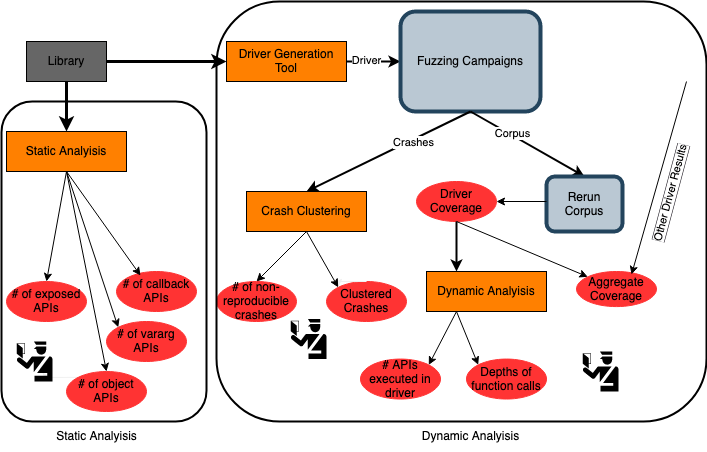
\includegraphics[width=16cm]{figures/framework.png}
	\caption{High-level overview}
	\label{fig:framework}
\end{figure}

\section{Design of the fuzzing campaigns}
Once the drivers have been compiled with the necessary
instrumentations, the fuzzing process can be initiated. 
However, before starting the fuzzing, there are two crucial
parameters that need to be considered: time and computational 
resources. These parameters play a significant role in determining
the efficiency and effectiveness of the fuzzing campaign.

Firstly, it is important to decide how many fuzzers should be 
run in parallel. It is recommended to choose the number of 
physical cores available minus one and assign each core to a 
specific fuzzer. This allows for optimal utilization of 
computational resources and ensures that the fuzzers can run 
concurrently without interference with each other.

Next, the duration for which the fuzzers should run needs to be 
determined. Time is a limited and valuable resource, and users 
need to set constraints based on their specific requirements. It
is essential to maintain consistency across different fuzzers 
generated from the same tool. When comparing different tools or 
manually written drivers, one approach is to define the total 
available time resource and allocate it proportionally among the 
fuzzers. For example, if a budget of 100 hours is defined, and a 
tool like UTopia generates 50 synthetic drivers while there are 10
manually written drivers in OSS-Fuzz, each UTopia fuzzer would run 
for 2 hours, and each OSS-Fuzz fuzzer would run for 10 hours. This
ensures a fair comparison and allows for an equal allocation of 
time resources among different fuzzers.

By carefully considering the number of parallelly running fuzzers 
and the allocated fuzzing time, users can optimize their fuzzing 
process to make the most efficient use of available computational
resources and ensure consistent evaluation of different fuzzers or
driver generation tools. 

Once the decisions regarding the number of parallel fuzzers and 
the allocated fuzzing time have been made, the fuzzing process 
can be initiated using LibFuzzer within isolated and constrained
Docker containers.

\lstset{caption={Full command for running LibFuzzer inside Docker container}, label=docker}
\begin{lstlisting}[language={c++}]
docker run \
--rm \
--cpuset-cpus $CPU_ID \
--shm-size=2g \
-d \
--name $fuzz_target \
-v $(pwd):/$target_tool \
-t $CONTAINER_NAME \
timeout $TIMEOUT $FUZZ_BINARY $CORPUS -fork=1 -ignore_timeouts=1 -ignore_crashes=1 -ignore_ooms=1 -artifact_prefix=$CRASHES
\end{lstlisting}


Upon completion of the fuzzing campaign, two relevant folders will
be obtained: "crashes" and "corpus". The "crashes" folder contains 
all the inputs that caused the fuzzer to crash during the fuzzing 
process. These inputs are particularly interesting as they may 
indicate potential vulnerabilities or bugs within the library.
On the other hand, the "corpus" folder contains all the inputs 
that the fuzzing engine found "interesting" based on coverage 
metrics. These inputs have contributed to achieving higher code 
coverage within the targeted library and may have triggered unique 
execution paths or uncovered previously unknown behaviors.

It is important to acknowledge that fuzzing is a probabilistic 
process, and the results obtained from a single fuzzing campaign
may not be representative of the overall performance of a fuzzer. 
To ensure statistically confident comparisons between any two 
given fuzzers based on specific metrics, it is recommended to run 
fuzzing campaigns multiple times, at least five.

\section{Crash clustering}
After fuzzing is over typically get a significant number of crashing inputs.
However, it is important to note that not all of these inputs necessarily
represent unique bugs within the target library. To address this issue, we 
use CASR \cite{casr}. CASR is a tool for determining the similarity 
between crashes by analyzing their respective call stacks. CASR can
effectively identify and eliminate duplicate crashes. The tool first 
focuses on removing duplicate crashes, ensuring that each unique crash is 
represented only once in the final set. Next, CASR uses a hierarchical 
clustering method to group the remaining crashes based on their
similarities, see figure \ref{fig:callstacks}. 

\begin{figure}[htb]
	\centering
	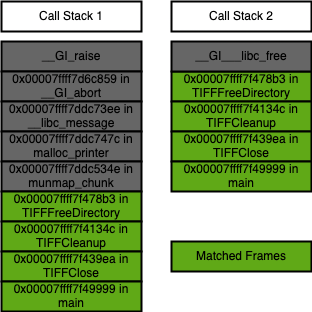
\includegraphics[]{figures/callstacks.png}
	\caption{Two crashes from the same cluster}
	\label{fig:callstacks}
\end{figure}

One metric that we aim to extract from the crash analysis step is the 
number of unreproducible crashes. These crashes occur when a driver fails 
to handle state resetting correctly, leading to inconsistent or 
unpredictable behavior during the fuzzing process. As LibFuzzer is an in-
process fuzzing engine, the state of the library is carried over between 
fuzzing iterations. If the driver does not reset its internal state 
properly after each fuzz input, it can result in unreproducible crashes.
Hence we can use this number to assess the quality of the driver as it 
shows how well the driver handles the state. 

The most straightforward way to get this number is to rerun the fuzzer with 
crashing inputs and see how many of them succeed. However, since CASR
already reruns these inputs, we might just parse the log file to find such
misleading inputs.

After deduplication and clustering are done, we are left with a number of
unique crashes. Unfortunately, a human analyst needs to go through these
inputs to determine whether it is a bug in a library or in a driver 
itself (false positive) and assess if it's an exploitable vulnerability.

\section{Coverage metrics}
The first step to getting coverage metrics is corpora minimization. Corpora 
minimization involves reducing the size of the initial corpus of interesting 
inputs generated during the fuzzing process. The purpose of corpora minimization 
is to remove redundant or unnecessary inputs while still preserving the coverage 
achieved by the remaining inputs. By eliminating redundant inputs, corpora 
minimization allows for more efficient analysis and exploration of the remaining inputs.

To minimize corpora, we will run the same LibFuzzer fuzzer with special \lstinline{-merge=1} 
flag: \\
\lstinline{mkdir corp_min && ./fuzzer -merge=1 ./corp_min ./corp_original}

Next, we need to compile the fuzz driver with coverage instrumentation flags 
and run this coverage-instrumented fuzzer (also known as profile) over the minimized corpora: \\
\lstinline{./fuzzer_cov_intrumented -runs=0 ./corp_min}

Once the fuzzer has completed iterating through all the inputs, it 
generates a .profraw file that contains highly accurate code coverage 
information. To extract the coverage metrics, the next step is to convert 
this .profraw file into a profile data file using the llvm-profdata tool \cite{profdata}. 
This tool processes the raw profile data and prepares it for further 
analysis. After obtaining the profile data file, we will use the llvm-
cov tool to extract various metrics of our fuzzing campaign. 
llvm-cov \cite{cov} provides a wide range of functionalities to analyze profile data 
files, including generating reports, identifying uncovered code regions, 
and calculating coverage percentages at different granularities such as 
basic blocks, functions, and lines. Scripts can be further adapted to
the user's concrete use case, for example, we can use the list of 
"challenging" APIs that we inferred during static analysis, to see
what percentage of them have been fuzzed.

\section{Driver Complexity}
To gain insights into how deeply fuzzer explores the library, we use GDB. 
From the previous step we already have coverage information, which
contains all the executed functions, we strategically place the breakpoints
at these function calls. Then we rerun the fuzzer and when breakpoints are hit,
we log the backtrace using gdb. By collecting stack trace dumps at various 
breakpoints, we obtain a nice view of the functions triggered by the fuzzer. 
This trace dump can be further processed to extract different metrics of
interest.

One important metric is the maximum depth reached by the fuzzer,
which indicates the furthest level of function calls from "LLVMFuzzOneInput".
This metric provides an understanding of the fuzzer's ability to explore
deeper levels of the library. Additionally, average depth provides
a measure of the overall depth of function calls. We can also combine
these metrics with per-function coverage to see how being deep in
the library correlates with how much the function is fuzzed.

Furthermore, by analyzing the stack trace dump, we can identify the 
APIs directly called within the driver code. 
This number will be dynamic and might not
represent the true value that can be obtained statically, however, we
argue that this is a more important metric, since for example tools
like FuzzGen are able to generate drivers with an arbitrary number of 
API calls, which makes static information useless for comparison. 
We currently do not infer this number statically, but it is planned 
to add that feature, since such information would be useful for
more flexible driver generation tools to create drivers that are 
similar to ones created by other tools for direct comparison. 


\begin{figure}[htb]
	\centering
	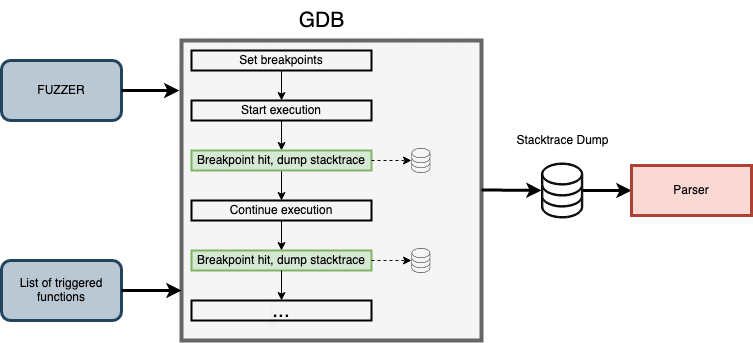
\includegraphics[width=16cm]{figures/stacktrace.png}
	\caption{Stacktrace analysis with GDB}
	\label{fig:stacktrace}
\end{figure}





% Present the results of your fuzzing campaigns, any vulnerabilities or bugs discovered.
% Compare the effectiveness and efficiency of automatic driver generation tools with manually written drivers.
% Discuss any insights or observations gained from the evaluation process.
%%%%%%%%%%%%%%%%%%%%
\chapter{Evaluation}
%%%%%%%%%%%%%%%%%%%%

\textbf{Evaluation Environment:} Describe the machine used. Set-up (single core per docker). Campaing length (1h). Etc.


One section for each experiment, ideally one per tool.


Utopia coverage with and without initial seeds.


1d heatmap: \url{https://stackoverflow.com/questions/45841786/creating-a-1d-heat-map-from-a-line-graph}

Klees. et al

TODO:
How does FuzzGen generate initial seeds? Maybe it's more effective to do it from
library consumers, rather than primitive constants that UTopia extracts from unit
tests.


Target analysis: \#apis exposed. callbacks? var args? objects?


Crashes, unique crashes, unreproducible crashes, false positives. 
Max depth of a fuzzer. \# of APIs, unique APIs used inside driver.
coverage metrics: basic blocks, \# functions / \#total. 
\# exposed APIs / \# total.







% Summarize the key findings and contributions of your project.
% Reflect on the strengths and limitations of the automatic driver generation tools and the evaluation tool.
% Discuss potential areas for further research and improvement.
%%%%%%%%%%%%%%%%%%%%
\chapter{Conclusion}
%%%%%%%%%%%%%%%%%%%%

We have explored the state-of-the-art in automatic driver generation
for library fuzzing, focusing on developing a methodology and framework
for evaluating synthetic drivers. We began by discussing the complexities 
of library fuzzing, including the need for the deep understanding of the 
library APIs, seed selection, callback handling, error handling, and 
state management. These challenges highlight the importance of 
developing automated solutions and represent the main issues these tools 
need to tackle. 

In conclusion, our project has demonstrated the value and potential 
of automatic driver generation for library fuzzing. We believe that 
our methodology and framework contribute to the advancement of 
software security practices, providing a more efficient and effective 
approach to library fuzzing.

\cleardoublepage
\phantomsection
\addcontentsline{toc}{chapter}{Bibliography}
\printbibliography

% Appendices are optional
% \appendix
% %%%%%%%%%%%%%%%%%%%%%%%%%%%%%%%%%%%%%%
% \chapter{How to make a transmogrifier}
% %%%%%%%%%%%%%%%%%%%%%%%%%%%%%%%%%%%%%%
%
% In case you ever need an (optional) appendix.
%
% You need the following items:
% \begin{itemize}
% \item A box
% \item Crayons
% \item A self-aware 5-year old
% \end{itemize}

\end{document}